\chapter{Resultados da Aplicação do \textit{Framework}}

Neste capítulo são apresentados os resultados de cada \textit{sprint} executada nos projetos selecionados para análise. Neste trabalho, cada \textit{sprint} representa um ciclo de pesquisa-ação e, como etapas de um ciclo, tem-se o planejamento, a ação e a avaliação. O relato da etapa de planejamento detalha tudo o que foi concebido entre a equipe de pesquisa, equipe de TI da instituição e área de negócio do projeto. A etapa ação evidencia como as atividades planejadas na etapa anterior se desenvolveram. Por fim, na etapa de avaliação, os dados coletados são exibidos bem como uma breve análise. Será possível contemplar gráficos comparativos ao final para evidenciar a evolução dos ciclos em cada projeto.

\section{Inicialização dos Ciclos - Treinamento}

Como demonstrado no planejamento da execução dos ciclos de pesquisa-ação, no capítulo sobre Materiais e Métodos, foi realizado um treinamento em todas as instituições com o propósito de esclarecer conceitos e práticas propostas pelo \textit{framework}. Nesse âmbito, foram evidenciados os aspectos inerentes à verificação de \textit{software} e utilização de ferramentas para as equipes de TI e, por outro lado, procurou-se dialogar com as áreas de negócio para tratar sobre os aspectos formais de como os projetos seriam executados a partir daquele momento, considerando práticas da VBSE.

Para familiarizar as equipes de TI com as práticas de implementação de testes unitários e inspeção de código, foram organizadas dinâmicas denominadas \textit{Coding Dojo}. Nesse tipo de dinâmica todas as pessoas atuam na construção de uma solução proposta pelo idealizador, alternando a posição reflexiva da platéia com as posições mais ativas dos pilotos. Assim, a construção sempre continua a partir do que os pilotos anteriores já desenvolveram.

As dinâmicas foram projetadas considerando as tecnologias e ferramentas utilizadas pelas equipes de TI. No caso da CGDF, para o projeto do Portal, considerou-se uma dinâmica de desenvolvimento de uma API \textit{REST} utilizando o \textit{framework Spring}. Adicionalmente, os participantes desenvolveram testes unitários e os demais desenvolvedores desempenhavam ações de inspeção. De forma semelhante, para o projeto de construção do Sistema de Ouvidoria foi organizada uma dinâmica para desenvolvimento de um simples exemplo com testes e inspeções. Para a equipe de desenvolvimento do Sistema de Correição não foi necessário promover outro treinamento, visto que os integrantes já haviam participado dos dojos anteriores.

No Laboratório Fábrica de \textit{Software} foi feito um dojo que envolvia a criação de uma aplicação \textit{mobile} na plataforma \textit{Android} juntamente com a implementação de testes unitários e inspeções.

Com relação às áreas de negócio, foi necessário enfatizar o motivo pelo qual a quantidade de \textit{story points} passou a ser menor: aumento da qualidade das entregas. Para executar as atividades de verificação de \textit{software}, as equipes de TI optaram, a priori, pela redução da carga de trabalho.

\section{Ciclo 1}

O principal objetivo do Ciclo 1 foi avaliar o primeiro uso do \textit{framework} de avaliação da qualidade de código nos contextos selecionados e, a partir dos resultados obtidos, caso necessário, efetuar ajustes nas atividades constituintes do mesmo. A seções a seguir descrevem de forma detalhada os acontecimentos e dados coletados durante a execução da \textit{sprint} 1 dos projetos selecionados.

\subsection{Portal da Transparência}

\subsubsection{Planejamento}

A partir de uma reunião com a área de negócio, tendo em vista o acordo de resultados com o governador do Distrito Federal, foi realizada uma priorização de itens do \textit{backlog}. Dessa forma, as seguintes funcionalidades foram acordadas:

\begin{itemize}
	\item Ajustes na consulta de Empresas Punidas
	\item Reformulação de filtros nos \textit{dashboards} de dados sobre Servidores e Remuneração dos Servidores
	\item Ajustes na consulta de Licitações e Contratos
\end{itemize}

Antes do início da \textit{Sprint} 1, os desenvolvedores configuraram o ambiente de testes, visto que o projeto do Portal não compreendia essas atividades anteriormente.

\subsubsection{Ação}

Com base nos itens do \textit{backlog} priorizados, todas as tarefas foram criadas na ferramenta de gerenciamento TFS. A partir de então, as atividades corriqueiras do \textit{Scrum} foram executadas em conjunto com as práticas propostas pelo \textit{framework} concebido neste trabalho.

\subsubsection{Avaliação}

A \textit{Sprint} 1 do projeto do portal foi executada com êxito. Todas as funcionalidades foram entregues. É válido ressaltar também que os testes unitários foram devidamente implementados para todos os componentes que sofreram alterações e também, as inspeções foram realizadas. Contudo, a equipe do projeto protelou as atividades de verificação, tornando a finalização da \textit{sprint} mais onerosa.

As tabelas \ref{table:tabela2} e \ref{table:tabela3} exibem um resumo das métricas coletadas para as camadas de \textit{frontend} e \textit{backend}, respectivamente.

\begin{table}[h]
\caption{Tabela Resumo - Métricas \textit{Sprint} 1 - Portal da Transparência (\textit{Frontend})}
\centering
\begin{tabular}{ | m{8cm} | m{8cm} | } 
\hline
Número de Defeitos & 4 \\ 
\hline
Taxa de Acertos por Linha de Código & 3 \\ 
\hline
\end{tabular}
\label{table:tabela2}
\end{table}

\begin{table}[h]
\caption{Tabela Resumo - Métricas \textit{Sprint} 1 - Portal da Transparência (\textit{Backend})}
\centering
\begin{tabular}{ | m{8cm} | m{8cm} | } 
\hline
Número de Defeitos & 3 \\ 
\hline
Taxa de Acertos por Linha de Código & 2 \\ 
\hline
\end{tabular}
\label{table:tabela3}
\end{table}

A partir dos dados exibidos pelas tabelas acima, considerando somente os novos trechos de códigos produzidos e os módulos alterados, as inspeções foram capazes de identificar 4 defeitos na camada \textit{frontend} e 3 defeitos na camada \textit{backend}. De fato, por mais que os desenvolvedores da equipe estivessem implementando de forma concisa, ainda foi possível contemplar defeitos no código. Ao final da \textit{sprint}, todos os defeitos foram corrigidos antes da mesclagem final.

Com relação à taxa de acertos por linha de código, a suíte de testes elaborada foi capaz de exercitar, em média, 3 vezes os trechos de código sob teste na camada \textit{frontend} e 2 vezes os trechos de código sob teste na camada \textit{backend}. Ao final da \textit{sprint} foi possível contemplar um percentual total de cobertura igual a 15,43\% na camada \textit{frontend} e 22,10\% na camada \textit{backend}.

Com relação à camada \textit{backend}, calculou-se o índice de manutenibilidade para todos os componentes alterados. A tabela \ref{table:tabela4} exibe estes dados, indicando a classe com o seu respectivo índice calculado.

\begin{table}[h]
\caption{Índice de Manutenibilidade \textit{Sprint} 1 - Portal da Transparência (\textit{Backend})}
\centering
\begin{tabular}{ | m{10cm} | m{6cm} | } 
\hline
Empresa Punida - Modelo & 95,12 \\ 
\hline
Empresa Punida - \textit{Controller} & 94,99 \\ 
\hline
Servidores - \textit{Controller} & 49,31 \\ 
\hline
Remuneração - \textit{Controller} & 74,51 \\ 
\hline
Empresa Punida Relatório - \textit{Service} & 84,82 \\
\hline
\end{tabular}
\label{table:tabela4}
\end{table}

Foi possível perceber um valor baixo do índice para a classe \textit{ServidoresController} tendo em vista os valores que as demais classes atingiram. Contudo, é um valor aceitável de acordo com os parâmetros da \textit{Microsoft} e indica a direção para futuros esforços em refatoração.

Com relação ao número de falhas identificadas pela área de negócio, nada foi reportado. Este aspecto indica que uma verificação concisa possui forte impacto na qualidade do produto entregue.

Por fim, tem-se o percentual obtido para as respostas relacionadas ao questionário de verificação da satisfação dos desenvolvedores ao utilizarem o \textit{framework}. Foi possível perceber que a equipe de desenvolvimento do portal apresentou boa aceitação quanto ao uso do \textit{framework}. Em linhas gerais, as inspeções e a forma de implementar testes unitários foram bem vistas pelos desenvolvedores. Ainda assim, as práticas propostas, segundo os desenvolvedores da equipe, se mostratam onerosas em contextos de equipes pequenas (até 3 desenvolvedores). A figura \ref{fig:satisfacaoPortal1} exibe a quantidade de respostas para cada questão do questionário de verificação da satisfação.

\begin{figure}[h]
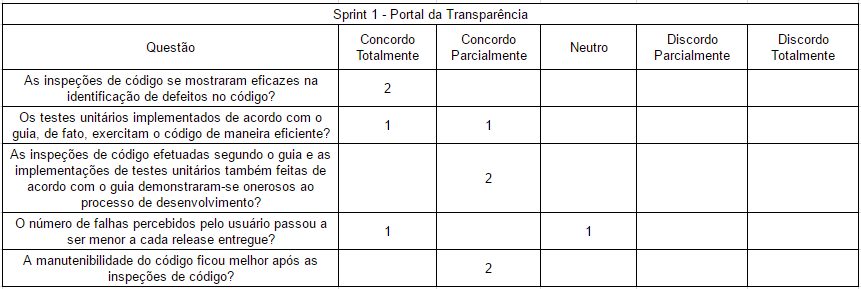
\includegraphics[width=\textwidth]{figuras/isd_portal_1.png}
\caption{Índice de Satisfação dos Desenvolvedores - \textit{Sprint} 1 do Portal}
\label{fig:satisfacaoPortal1}
\end{figure}

\clearpage

\subsection{Sistema de Ouvidoria}

\subsubsection{Planejamento}

Assim como o projeto do Portal, o Sistema de Ouvidoria é um projeto que possui metas no acordo de resultados com o governador do Distrito Federal. Por se tratar de um sistema que recebe diretamente manifestações por parte dos cidadãos e por armazenar tantos dados diariamente, as seguintes funcionalidades foram acordadas:

\begin{itemize}
	\item Reformulação do filtro de manifestações
	\item Disponibilização de um questionário de pesquisa de satisfação dos cidadãos quanto ao atendimento das manifestações
\end{itemize}

Como o projeto não compreendia práticas de verificação de \textit{software}, a equipe de TI também teve que configurar o ambiente de testes antes do início da \textit{sprint}.

\subsubsection{Ação}

As atividades padrão do \textit{Scrum} e do \textit{framework} aqui proposto foram desenvolvidas durante a \textit{sprint}. Adicionalmente, todas as tarefas relacionadas às funcionalidades foram criadas no TFS para maior controle do andamento da iteração de desenvolvimento.

\subsubsection{Avaliação}

Assim como no projeto do portal, a primeira \textit{sprint} do projeto do sistema de ouvidoria também foi executada com êxito. A equipe de desenvolvimento também protelou as atividades de verificação, alocando-as para o final da \textit{sprint}.

A tabela \ref{table:tabela5} exibe um resumo das métricas coletadas para as camadas de \textit{backend}.

\begin{table}[h]
\caption{Tabela Resumo - Métricas \textit{Sprint} 1 - Sistema de Ouvidoria (\textit{Backend})}
\centering
\begin{tabular}{ | m{8cm} | m{8cm} | } 
\hline
Número de Defeitos & 1 \\ 
\hline
Taxa de Acertos por Linha de Código & 3 \\ 
\hline
\end{tabular}
\label{table:tabela5}
\end{table}

A partir dos dados exibidos pela tabela, constata-se que o código foi bem implementado, tendo em vista o baixo número de defeitos identificados durante a inspeção. Adicionalmente, a suíte de testes foi capaz de exercitar, em média, 3 vezes o trecho de código sob teste. A cobertura final contemplada na camada de \textit{backend} foi igual a 23,88\%.

Com relação ao índice de manutenibilidade, os valores calculados são expressos na tabela \ref{table:tabela6}.

\begin{table}[h]
\caption{Índice de Manutenibilidade \textit{Sprint} 1 - Sistema de Ouvidoria (\textit{Backend})}
\centering
\begin{tabular}{ | m{12cm} | m{4cm} | } 
\hline
\textit{CoreAppService} - \textit{OuvCidadania.AppService} & 61 \\ 
\hline
Resposta - \textit{Domain.Entity} & 90 \\ 
\hline
Resposta Questionário - \textit{Domain.Entity} & 90 \\ 
\hline
Resposta Exception - \textit{Domain.Exceptions} & 98 \\ 
\hline
IRespostaRepository - \textit{Domain.Repository} & 100 \\
\hline
IRespostaQuestionarioService - \textit{Domain.Service} & 100 \\
\hline
IRespostaService - \textit{Domain.Service} & 100 \\
\hline
Resposta Questionario Service - \textit{Domain.Service} & 65 \\
\hline
Resposta Service - \textit{Domain.Service} & 64 \\
\hline
\end{tabular}
\label{table:tabela6}
\end{table}

\hfill \break

Considerando os parâmetros da \textit{Microsoft}, todas as classes e interfaces apresentaram índices de manutenibilidade aceitáveis. Contudo, deve-se atentar para as classes na camada de serviço, que indicam necessidade de refatorações para que o índice de manutenibilidade possa aumentar.

Assim como no projeto do portal, não houve registro de falhas por parte da área de negócio. Todas as funcionalidades entregues ao final da \textit{sprint} foram estabelecidas de forma consistente.

Por fim, com relação ao índice de satisfação dos desenvolvedores, também contemplou-se uma boa percepção acerca da utilização do \textit{framework}. A equipe também considerou as práticas propostas pelo \textit{framework} onerosas para contextos de equipes pequenas e sugeriu que fosse feita uma adequação das práticas para equipes pequenas. A figura \ref{fig:satisfacaoOuvidoria1} exibe a quantidade de respostas para cada questão do questionário de verificação da satisfação.

\begin{figure}[h]
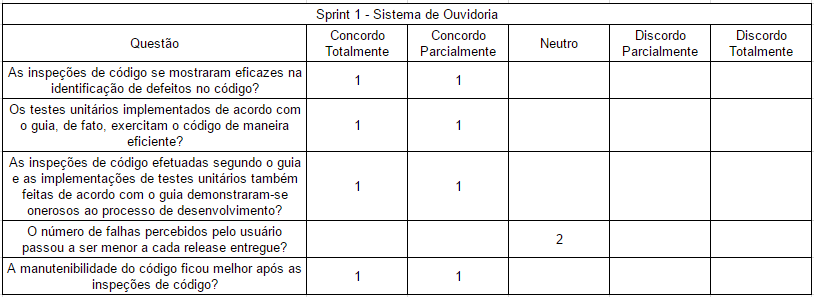
\includegraphics[width=\textwidth]{figuras/isd_ouvdf_1.png}
\caption{Índice de Satisfação dos Desenvolvedores - \textit{Sprint} 1 do Sistema de Ouvidoria}
\label{fig:satisfacaoOuvidoria1}
\end{figure}

\clearpage

\subsection{SICOR - Sistema de Correição}

\subsubsection{Planejamento}

Pelo fato de o SICOR ser um novo projeto na CGDF, a equipe de TI realizou um diálogo prévio com a área de negócio para obter uma visão geral acerca de todas as funcionalidades que o sistema deveria possuir até a data da primeira entrega prevista no acordo de resultados com o governador.

Foi possível perceber a necessidade de agrupar as funcionalidades do sistema em 4 \textit{features} principais, sendo:

\begin{itemize}
	\item Módulo Administrativo
	\item Módulo Correcional
	\item Módulo Disciplinar
	\item Módulo de Responsabilização
\end{itemize}

Considerando os aspectos da VBSE, durante as conversas com a área de negócio, percebeu-se que todas as informações presentes no sistema deveriam ser tratadas como sigilosas. Adicionalmente, a área de negócio solicitou uma trilha de auditoria complexa para a aplicação, sendo que todos os eventos ocorridos deveriam ser registrados e sempre vinculados ao usuário responsável pelo mesmo.

Dessa forma, a área de negócio priorizou o módulo adminstrativo, caracterizando-o como crítico e fundamental para o sistema. Adicionalmente, a equipe de TI ponderou que este módulo seria fundamental para inicializar a construção da arquitetura do sistema, visto que todos os mecanismos de segurança e registro de eventos deveriam ser projetados e implementados logo no início.

Para a primeira \textit{sprint} do projeto, as funcionalidades acordadas foram:

\begin{itemize}
	\item Criação da arquitetura de registro de eventos (Logs)
	\item Cadastro de Usuários
	\item Cadastro de Unidades
	\item Login
	\item Cadastro de Perfis
\end{itemize}

Após priorização, a equipe de desenvolvimento iniciou as configurações de ambiente, banco de dados etc. O mais interessante é que a reestruturação efetuada nos outros projetos contribuiu de forma significativa para o início da contrução do SICOR. Além disso, a equipe de desenvolvimento já havia participado previamente das iterações de desenvolvimento de outros projetos e, portanto, já estava familiarizada com as práticas propostas pelo \textit{framework} de avaliação da qualidade de código.

\subsubsection{Ação}

Antes que a \textit{sprint} fosse iniciada, todas as histórias foram registradas no TFS. Adicionalmente, todas as tarefas vinculadas também foram cadastradas. Ao final da execução da \textit{sprint}, somente uma funcionalidade não foi entregue, sendo o cadastro de unidades.

\subsubsection{Avaliação}

Apesar de uma funcionalidade não ter sido entregue, a primeira \textit{sprint} do SICOR foi considerada um sucesso. As tabelas \ref{table:tabela7} e \ref{table:tabela8} exibem um resumo das métricas coletadas para as camadas de \textit{frontend} e \textit{backend}, respectivamente.

\begin{table}[h]
\caption{Tabela Resumo - Métricas \textit{Sprint} 1 - SICOR (\textit{Frontend})}
\centering
\begin{tabular}{ | m{8cm} | m{8cm} | } 
\hline
Número de Defeitos & 1 \\ 
\hline
Taxa de Acertos por Linha de Código & 1 \\ 
\hline
\end{tabular}
\label{table:tabela7}
\end{table}

\begin{table}[h]
\caption{Tabela Resumo - Métricas \textit{Sprint} 1 - SICOR (\textit{Backend})}
\centering
\begin{tabular}{ | m{8cm} | m{8cm} | } 
\hline
Número de Defeitos & 1 \\ 
\hline
Taxa de Acertos por Linha de Código & 2,46 \\ 
\hline
\end{tabular}
\label{table:tabela8}
\end{table}

A partir dos dados exibidos nas tabelas acima é possível perceber uma baixa quantidade de defeitos, que evidencia uma maior precisão por parte dos desenvolvedores nos momentos de implementação. Adicionalmente, a suíte de testes unitários implementada foi capaz de exercitar, em média, 1 vez o trecho de código sob teste na camada de \textit{frontend} e 2,46 vezes o trecho de código sob teste na camada de \textit{backend}. Ao final da \textit{sprint}, percebeu-se um percentual total de cobetura igual a 100\% na camada de \textit{frontend} e 95\% na camada de \textit{backend}. É válido ressaltar que não foi reportado nenhuma percepção de falha do sistema por parte da área de negócio durante a homologação.

Com relação ao quesito manutenibilidade e complexidade do código, como mencionado no capítulo sobre metodologia, adotou-se a métrica Flog (devido às particularidades da linguagem Ruby e do \textit{framework Rails}). A seguir, tem-se a tabela \ref{table:tabela9}, que exibe a pontuação total da métrica para as principais classes implementadas.

\begin{table}[h]
\caption{Flog \textit{Sprint} 1 - SICOR (\textit{Backend})}
\centering
\begin{tabular}{ | m{12cm} | m{4cm} | } 
\hline
Auditoria (Log) & 14 \\ 
\hline
\textit{Application} - \textit{Controller} & 12 \\ 
\hline
Usuário - \textit{Controller} & 38 \\ 
\hline
Usuário - Modelo & 11,6 \\ 
\hline
Órgão - \textit{Controller} & 3,2 \\
\hline
Auditoria Base - Módulo Log & 3 \\
\hline
\textit{Handler} - Módulo Usuário & 2,3 \\
\hline
\end{tabular}
\label{table:tabela9}
\end{table}

\clearpage

Embora a trilha de auditoria realmente tenha sido considerada uma funcionalidade crítica do sistema, as escolhas de tecnologias se caracterizaram como apropriadas para o contexto, visto que o processamento é dividido entre o cliente e o servidor (API \textit{REST} com cliente \textit{AngularJS}). Esse aspecto favoreceu a diminuição da complexidade do código na camada de \textit{backend}.

Por fim, é válido ressaltar que embora os desenvolvedores do projeto já tivessem familiaridade com o \textit{framework} de avaliação da qualidade de código, ainda consideraram as práticas onerosas para o processo de desenvolvimento em contextos de equipes pequenas. Contudo, afirmaram que se a equipe possuir disciplina no seu fluxo de atividades, é possível conciliar o alto número de atividades com os prazos. A figura \ref{fig:satisfacaoSicor1} exibe a quantidade de respostas para cada questão do questionário de verificação da satisfação.

\begin{figure}[h]
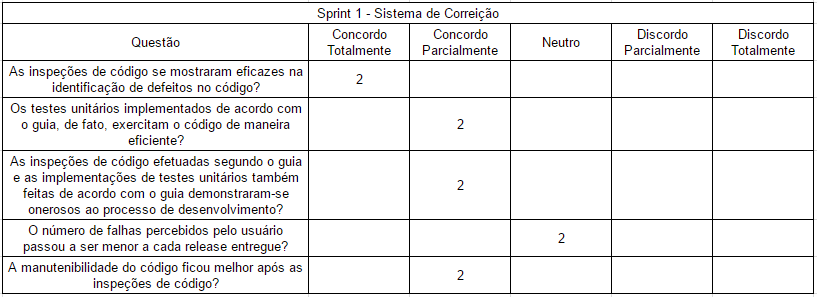
\includegraphics[width=\textwidth]{figuras/isd_sicor_1.png}
\caption{Índice de Satisfação dos Desenvolvedores - \textit{Sprint} 1 do SICOR}
\label{fig:satisfacaoSicor1}
\end{figure}

\clearpage

\subsection{Sistema de Perícia Médica}

\subsubsection{Planejamento}

Durante os diálogos realizados entre a equipe de desenvolvimento e a área de negócio, o projeto de desenvolvimento do Sistema de Perícia Médica esteve voltado, durante a primeira \textit{sprint} avaliada por este trabalho, para aperfeiçoamentos e correções de \textit{bugs} encontrados nas funcionalidades desenvolvidas nas iterações precedentes.

Basicamente, os seguintes itens foram acordados com a área de negócio:

\begin{itemize}
	\item Melhorias no \textit{layout} da Aplicação \textit{Mobile}
	\item Aperfeiçoamentos no menu de operações disponíveis na Aplicação \textit{Mobile}
	\item Correção de bugs no cadastro de colaboradores
	\item Melhorias no cadastro de tablets na Aplicação \textit{Web}
\end{itemize}

\subsubsection{Ação}

Ao final da priorização, a equipe de desenvolvimento registrou as descrições dos itens a serem implementados bem como suas respectivas tarefas na ferramenta TFS. A \textit{sprint} contemplou atrasos, dessa forma, as atividades de verificação foram proteladas para o final da mesma, assim como as mesclagens de código considerando o fluxo e política de \textit{branches}.

\subsubsection{Avaliação}

Embora atrasos tenham sido contemplados, todas os itens tiveram sua implementação finalizada. A suíte de testes unitários implementada não contemplou todos os cenários mais básicos considerando a estrutura do código das classes. Adicionalmente, a equipe apresentou muita dificuldade para implementar testes de \textit{Fragments} (um dos elementos constituintes da arquitetura de uma aplicação para plataforma \textit{Android}) e assim, somente as classes da camada \textit{controller} foram finalizadas com suítes de testes consistentes. Quanto à aplicação \textit{Web}, as implementações ocorreram sem registro de dificuldades.

Considerando o código das aplicações, após as inspeções, foi contemplado um total de 5 defeitos. Pelo fato de ter ocorrido atrasos na execução da \textit{sprint}, os defeitos foram corrigidos após finalização da mesma e antes de ocorrer a entrega formal dos resultados para a área de negócio. Quanto a suíte de testes, cada método de teste foi capaz de exercitar somente 1 vez o trecho de código sob teste. Adicionalmente, a inexistência de uma ferramenta de análise de cobertura prejudicou a percepção de mais cenários de teste por parte da equipe de desenvolvimento.

Embora a suíte de testes não tenha sido implementada da melhor forma possível, a área de negócio não reportou nenhuma falha quanto ao que havia sido implementado.

Por fim, coletou-se o índice de manutenibilidade das classes alteradas durante a execução da \textit{sprint}. A tabela \ref{table:tabela10} exibe os resultados da coleta.

\begin{table}[h]
\caption{Índice de Manutenibilidade \textit{Sprint} 1 - Sistema de Perícia Médica (\textit{Backend})}
\centering
\begin{tabular}{ | m{12cm} | m{4cm} | } 
\hline
AlterarFuncaoFragment - \textit{Mobile} & 59 \\ 
\hline
MenuCoordenadorFragment - \textit{Mobile} & 64 \\ 
\hline
ColaboradorController - \textit{Mobile} & 73 \\ 
\hline
ColaboradorDAO - \textit{Mobile} & 69 \\ 
\hline
CadastrarColaboradorFragment - \textit{Mobile} & 53 \\
\hline
MainActivity - \textit{Mobile} & 73 \\
\hline
ViewUtils - \textit{Mobile} & 59 \\
\hline
ListarEquipeContratanteFragment - \textit{Mobile} & 63 \\
\hline
TabletController - \textit{Web} & 74 \\
\hline
SessaoController - \textit{Web} & 65 \\
\hline
LiberaQRCodeController - \textit{Web} & 72 \\
\hline
RegistrarTabletEvento - \textit{Web Service} & 71 \\
\hline
\end{tabular}
\label{table:tabela10}
\end{table}

É possível perceber com os dados da tabela acima que as classes apresentaram índice de manutenibilidade aceitável dentro dos parâmetros da \textit{Microsoft}. Como mencionado anteriormente, mesmo que a suíte de testes não tenha contemplado todos os cenários básicos possíveis, as inspeções auxiliaram na identificação de defeitos e na visualização de formas melhores de se organizar o código, possibilitando altos índices de manutenibilidade e número reduzido de falhas.

Com relação ao uso do \textit{framework}, a equipe do Laboratório Fábrica de \textit{Software} apresentou menos receptividade do que as equipes da CGDF. Contudo, ainda assim, ressaltou que as inspeções auxiliaram significativamente na melhoria do índice de manutenibilidade do código. A figura \ref{fig:satisfacaoPericia1} exibe a quantidade de respostas para cada questão do questionário de verificação da satisfação.

\begin{figure}[h]
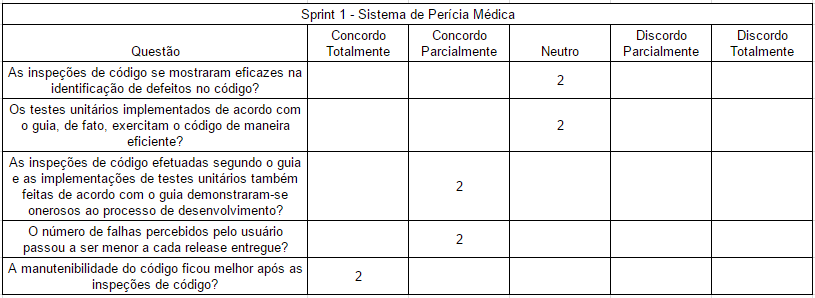
\includegraphics[width=\textwidth]{figuras/isd_pericia_1.png}
\caption{Índice de Satisfação dos Desenvolvedores - \textit{Sprint} 1 do Sistema de Perícia Médica}
\label{fig:satisfacaoPericia1}
\end{figure}

\clearpage

\section{Ciclo 2}

O principal objetivo do Ciclo 2 foi efetuar os ajustes necessários na execução das atividades propostas pelo \textit{framework} de avaliação da qualidade de código, bem como fornecer uma orientação quanto às dúvidas remanescentes por parte das equipes de desenvolvimento das instituições selecionadas para este trabalho.

Com base no relato do Ciclo 1, foi possível perceber que todas as equipes mencionaram que as práticas propostas pelo \textit{framework} se mostraram parcialmente onerosas ao processo de desenvolvimento em âmbito de equipes pequenas. Assim, procurou-se obter por parte dos desenvolvedores sugestões de melhoria para o fluxo proposto pelo \textit{framework}. Chegou-se a conclusão de que não poderia ocorrer exclusão de atividades mesmo para contextos menores, visto que o diferencial do \textit{framework} é justamente o agrupamento das melhores práticas relativas à implementação de testes unitários e realização de inspeções de código, bem como a incorporação dos conceitos da VBSE, possibilitando com que o projeto seja executado de forma a atingir sua missão.

As demais atividades do \textit{framework} apenas refletem o que já é proposto pelo \textit{Scrum}. Quanto à primeira atividade, relacionada à VBSE (Elicitação das Propostas de Valor), não percebeu-se nenhuma carga extra de trabalho. Inclusive, as áreas de negócio passaram a fornecer \textit{feedbacks} que expressavam maior satisfação quanto às atividades desempenhadas pelas equipes de desenvolvimento.

Considerando os fatos citados acima, as próprias equipes de desenvolvimento reconheceram que protelavam as atividades de verificação e que, pelo fato de não terem a cultura de realizar tais atividades, obtiveram certa dificuldade. Dessa maneira, nenhum ajuste foi efetuado no \textit{framework} e as equipes procuraram realizar as atividades com o mínimo de protelação durante o Ciclo 2.

\subsection{Portal da Transparência}

\subsubsection{Planejamento}

Em reunião com a área de negócio, considerando o acordo de resultados com o governador, as seguintes funcionalidades foram acordadas:

\begin{itemize}
	\item Reformulação da Consulta de Empresas Punidas (Compatibilização com os dados da CGU - Controladoria Geral da União)
	\item Inclusão da Consulta de Órgãos Deliberativos
	\item Aperfeiçoamentos na Consulta Dinâmica de Despesas
\end{itemize}

Antes do início da \textit{sprint}, a equipe não precisou dedicar tempo à configuração de ambiente de testes, visto que tudo foi feito durante a \textit{sprint} 1. Adicionalmente, a equipe de desenvolvimento acordou que nenhuma classe deveria ficar com índice de manutenibilidade inferior à 45 após finalização das implementações.

\subsubsection{Ação}

Com base nos itens do \textit{backlog} priorizados, todas as tarefas foram criadas na ferramenta de gerenciamento TFS. A partir de então a equipe de desenvolvimento passou a fornecer maior atenção para as atividades de verificação e sempre que uma funcionalidade era finalizada, imediatamente após ocorria a inspeção da mesma. Dessa forma, a \textit{sprint} foi executada com êxito dentro do prazo estabelecido.

\subsubsection{Avaliação}

A \textit{Sprint} 2 do projeto do portal, como mencionado na seção anterior, foi executada com êxito. Todas as funcionalidades foram entregues. É válido ressaltar também que os testes unitários foram devidamente implementados para todos os componentes que sofreram alterações e também, as inspeções foram realizadas.

As tabelas \ref{table:tabela11} e \ref{table:tabela12} exibem um resumo das métricas coletadas para as camadas de \textit{frontend} e \textit{backend}, respectivamente.

\begin{table}[h]
\caption{Tabela Resumo - Métricas \textit{Sprint} 2 - Portal da Transparência (\textit{Frontend})}
\centering
\begin{tabular}{ | m{8cm} | m{8cm} | } 
\hline
Número de Defeitos & 1 \\ 
\hline
Taxa de Acertos por Linha de Código & 4 \\ 
\hline
\end{tabular}
\label{table:tabela11}
\end{table}

\begin{table}[h]
\caption{Tabela Resumo - Métricas \textit{Sprint} 2 - Portal da Transparência (\textit{Backend})}
\centering
\begin{tabular}{ | m{8cm} | m{8cm} | } 
\hline
Número de Defeitos & 2 \\ 
\hline
Taxa de Acertos por Linha de Código & 2 \\ 
\hline
\end{tabular}
\label{table:tabela12}
\end{table}

A partir dos dados exibidos pelas tabelas acima, considerando somente os novos trechos de códigos produzidos e os módulos alterados, as inspeções foram capazes de identificar 1 defeito na camada \textit{frontend} e 2 defeitos na camada \textit{backend}. Ao final da \textit{sprint}, todos os defeitos foram corrigidos antes da mesclagem final.

Quanto à taxa de acertos por linha de código, a suíte de testes elaborada foi capaz de exercitar, em média, 4 vezes os trechos de código sob teste na camada \textit{frontend} e 2 vezes os trechos de código sob teste na camada \textit{backend}. Ao final da \textit{sprint} foi possível contemplar um percentual total de cobertura igual a 23,00\% na camada \textit{frontend} e 27,10\% na camada \textit{backend}.

Analisando de forma rápida os percentuais de cobertura, percebe-se que o aumento foi pouco expressivo. Contudo, a suíte de testes elaborada caracterizou-se como consistente ao final da \textit{sprint} 2, sendo que todos os cenários mais básicos para os módulos sob teste foram implementados.

Com relação à camada \textit{backend}, calculou-se o índice de manutenibilidade para todos os componentes alterados. A tabela \ref{table:tabela13} exibe estes dados, indicando a classe com o seu respectivo índice calculado.

\begin{table}[h]
\caption{Índice de Manutenibilidade \textit{Sprint} 2 - Portal da Transparência (\textit{Backend})}
\centering
\begin{tabular}{ | m{10cm} | m{6cm} | } 
\hline
Empresa Punida - Modelo & 77,32 \\ 
\hline
Empresa Punida - \textit{Controller} & 85,20 \\ 
\hline
Empresa Punida - \textit{Service} & 78,38 \\ 
\hline
Empresa Punida Relatório - \textit{Service} & 77,45 \\ 
\hline
Órgãos Deliberativos - Modelo & 80,46 \\
\hline
Prestando Contas - \textit{Controller} & 56,71 \\
\hline
Prestando Contas - \textit{Service} & 45,66 \\
\hline
Prestando Contas Relatório - \textit{Controller} & 84,72 \\
\hline
Prestando Contas Relatório - \textit{Service} & 77,17 \\
\hline
Consulta Dinâmica Despesa - Modelo & 68,62 \\
\hline
Despesa - \textit{Controller} & 49,71 \\
\hline
\end{tabular}
\label{table:tabela13}
\end{table}

Foi possível perceber índices de manutenibilidade dentro dos padrões estabelecidos pela \textit{Microsoft} e também, dentro da meta estabelecida pela equipe de desenvolvimento antes do início da \textit{sprint} 2. Algumas classes tiveram uma redução no índice de manutenibilidade pelo fato de que código foi acrescentado. Contudo, essa redução não se caracterizou como impactante para a qualidade em um primeiro momento. O que deve ser observado é a evolução futura desse quadro. Se o índice de manutenibilidade de uma determinada classe diminuir a cada \textit{sprint}, deverá ser feita uma refatoração.

Com relação ao número de falhas identificadas pela área de negócio, nada foi reportado. Este aspecto indica que uma verificação concisa possui forte impacto na qualidade do produto entregue.

Por fim, tem-se as respostas relacionadas ao questionário de verificação da satisfação dos desenvolvedores ao utilizarem o \textit{framework}. Percebeu-se maior aceitação e entendimento da importância das práticas da verificação de \textit{software} para obtenção de um produto com qualidade. A figura \ref{fig:satisfacaoPortal2} exibe a quantidade de respostas para cada questão do questionário de verificação da satisfação.

\begin{figure}[h]
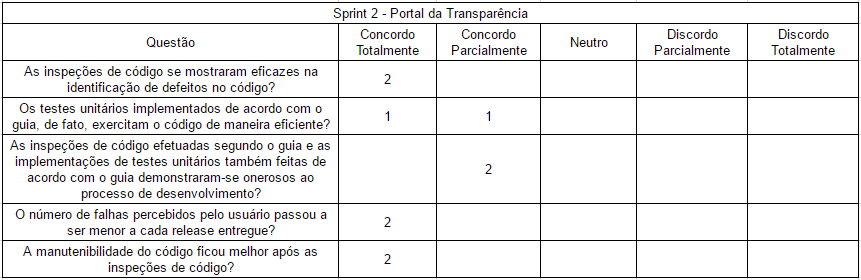
\includegraphics[width=\textwidth]{figuras/isd_portal_2.png}
\caption{Índice de Satisfação dos Desenvolvedores - \textit{Sprint} 2 do Portal}
\label{fig:satisfacaoPortal2}
\end{figure}

\clearpage

\subsection{SICOR - Sistema de Correição}

\subsubsection{Planejamento}

Em conversa com a área de negócio, as seguintes funcionalidades foram acordadas:

\begin{itemize}
	\item {Inclusão de Documento Originário}
	\item {Consulta de Documentos}
	\item {Exclusão de Documentos}
	\item {Alteração de Documentos}
	\item {Cadastro de Unidades - Pendência da \textit{Sprint} 1}
\end{itemize}

As funcionalidades descritas acima caracterizam-se como o núcleo do Módulo Correcional, visto que todas as denúncias que chegam à SUCOR são por meio de documentos originários. Adicionalmente, a primeira \textit{sprint} favoreceu a escolha destes itens, pois toda a estrutura já estava implementada.

\subsubsection{Ação}

Após priorização junto a área de negócio, a equipe de desenvolvimento registrou todas as tarefas relativas à implementação das funcionalidades no TFS. Adicionalmente, a equipe procurou estabelecer mais prioridades quanto à implementação de testes unitários. Pelo fato de terem sido alocados operações elementares, somente os testes para os módulos mais críticos foram desenvolvidos. Assim, a \textit{sprint} foi executada com êxito, entregando tudo que foi acordado.

\subsubsection{Avaliação}

Como mencionado na seção anterior, a \textit{sprint} 2 do projeto SICOR foi executada com êxito. As tabelas \ref{table:tabela14} e \ref{table:tabela15} exibem um resumo das métricas coletadas para as camadas de \textit{frontend} e \textit{backend}, respectivamente.

\begin{table}[h]
\caption{Tabela Resumo - Métricas \textit{Sprint} 2 - SICOR (\textit{Frontend})}
\centering
\begin{tabular}{ | m{8cm} | m{8cm} | } 
\hline
Número de Defeitos & 0 \\ 
\hline
Taxa de Acertos por Linha de Código & 2 \\ 
\hline
\end{tabular}
\label{table:tabela14}
\end{table}

\begin{table}[h]
\caption{Tabela Resumo - Métricas \textit{Sprint} 2 - SICOR (\textit{Backend})}
\centering
\begin{tabular}{ | m{8cm} | m{8cm} | } 
\hline
Número de Defeitos & 0 \\ 
\hline
Taxa de Acertos por Linha de Código & 2,76 \\ 
\hline
\end{tabular}
\label{table:tabela15}
\end{table}

A partir dos dados exibidos nas tabelas acima é possível perceber uma baixa quantidade de defeitos, que evidencia uma maior precisão por parte dos desenvolvedores nos momentos de implementação. Adicionalmente, a suíte de testes unitários implementada foi capaz de exercitar, em média, 2 vezes o trecho de código sob teste na camada de \textit{frontend} e 2,76 vezes o trecho de código sob teste na camada de \textit{backend}. Ao final da \textit{sprint}, percebeu-se um percentual total de cobetura igual a 73,86\% na camada de \textit{frontend} e 60\% na camada de \textit{backend}. É válido ressaltar que não foi reportado nenhuma percepção de falha do sistema por parte da área de negócio durante a homologação.

Embora o percentual total de cobertura tenha diminuído, percebe-se que a suíte de testes ainda caracteriza-se como consistente, visto que o número de acertos por linha de código aumentou. Como mencionado anteriormente, a redução do percentual deve-se ao aumento de linhas de código. De forma geral, à medida em que o projeto cresce, mais difícil é manter o percentual de 100\% de cobertura. Outro aspecto é que uma cobertura integral traz maior custo de desenvolvimento. Assim, é necessário ser mais seletivo quando se implementa testes unitários.

Com relação ao quesito manutenibilidade e complexidade do código, coletou-se a métrica Flog. A seguir, tem-se a tabela \ref{table:tabela16}, que exibe a pontuação total da métrica para as principais classes implementadas.

\begin{table}[h]
\caption{Flog \textit{Sprint} 2 - SICOR (\textit{Backend})}
\centering
\begin{tabular}{ | m{12cm} | m{4cm} | } 
\hline
Documento - \textit{Controller} & 57,3 \\ 
\hline
Documento - Modelo & 44,1 \\ 
\hline
Criar Documento - \textit{Service} & 17,3 \\ 
\hline
Atualizar Documento - \textit{Service} & 7,1 \\ 
\hline
Pesquisar Documento - \textit{Service} & 29,6 \\
\hline
\end{tabular}
\label{table:tabela16}
\end{table}

Com base nos dados apresentados pela tabela acima, percebe-se baixas pontuações de complexidade. Mesmo nas classes que apresentaram pontuações totais acima de 40, a média para os métodos da classe foi inferior à 8.

Por fim, tem-se as respostas relacionadas ao questionário de verificação da satisfação dos desenvolvedores ao utilizarem o \textit{framework}. Assim como no projeto do Portal, percebeu-se maior aceitação e entendimento da importância das práticas da verificação de \textit{software} para obtenção de um produto com qualidade. A figura \ref{fig:satisfacaoSicor2} exibe a quantidade de respostas para cada questão do questionário de verificação da satisfação.

\begin{figure}[h]
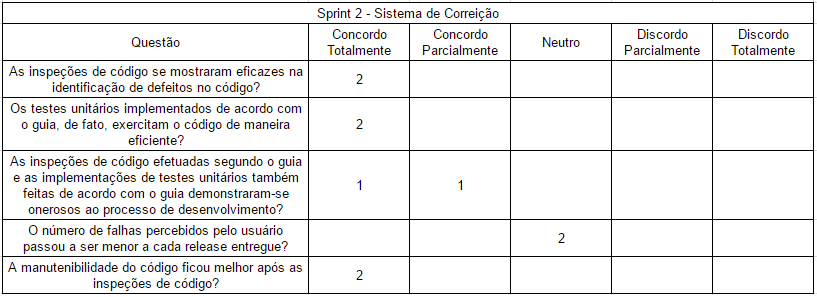
\includegraphics[width=\textwidth]{figuras/isd_sicor_2.png}
\caption{Índice de Satisfação dos Desenvolvedores - \textit{Sprint} 2 do SICOR}
\label{fig:satisfacaoSicor2}
\end{figure}

\clearpage

\subsection{Sistema de Perícia Médica}

\subsubsection{Planejamento}

A segunda iteração de desenvolvimento do projeto de construção do Sistema de Perícia Médica teve enfoque na sincronização de dados entre os \textit{tablets} portadores da aplicação. Esse mecanismo é fundamental para os testes de aptidão promovidos pela Instituição X, parceira e patrocinadora do Laboratório Fábrica de \textit{Software}.

As funcionalidades discutidas e acordadas entre a área de negócio e a área de desenvolvimento foram:

\begin{itemize}
	\item Criptografia do banco de dados da aplicação \textit{mobile}
	\item Registro de log de operações efetuadas na aplicação \textit{mobile}
	\item Transmissão de informações entre \textit{tablets}
	\item Mesclagem de dados a partir da compração do horário da alteração
\end{itemize}

\subsubsection{Ação}

Assim como em todas as iterações relatadas até a presente seção, a equipe de desenvolvimento registrou as atividades na ferramenta TFS para gerenciamento e controle do andamento da \textit{sprint}. Ao final, somente a funcionalidade de mesclagem de dados obteve testes unitários implementados. Nas demais, os módulos foram implementados, mas não tiveram testes unitários. As inspeções foram efetuadas em todos os módulos.

\subsubsection{Avaliação}

A partir das inspeções efetuadas pela equipe, foi identificado um total de 4 defeitos no código. Os defeitos foram corrigidos somente após o prazo de encerramenta da \textit{sprint}. Da mesma forma como na \textit{sprint} 1, a suíte de testes não se caracterizou como consistente a partir de uma perspectiva geral. Muitos testes não foram implementados e os módulos que obtiveram implementação de testes unitários careciam de mais cenários.

De forma semelhante à \textit{sprint} 1, a área de negócio não contemplou falhas durante a homologação dos itens desenvolvidos.

Por fim, coletou-se o índice de manutenibilidade das classes alteradas durante a execução da \textit{sprint}. A tabela \ref{table:tabela17} exibe os resultados da coleta.

\begin{table}[h]
\caption{Índice de Manutenibilidade \textit{Sprint} 2 - Sistema de Perícia Médica (\textit{Backend})}
\centering
\begin{tabular}{ | m{12cm} | m{4cm} | } 
\hline
ColaboradorDAO - \textit{Mobile} & 66 \\ 
\hline
CandidatoDAO - \textit{Mobile} & 70 \\
\hline
EquipeContratanteDAO - \textit{Mobile} & 66 \\
\hline
MembroEquipeContratanteDAO - \textit{Mobile} & 67 \\
\hline
InscritoDAO - \textit{Mobile} & 67 \\
\hline
ResultadoDAO - \textit{Mobile} & 67 \\
\hline
MiniBanco - \textit{Mobile} & 56 \\
\hline
\end{tabular}
\label{table:tabela17}
\end{table}

\clearpage

A partir dos dados apresentados pela tabela acima, é possível concluir que as inspeções auxiliaram na estabilidade do índice de manutenibilidade e favoreceu o aumento deste para algumas classes tendo em vista o índice de manutenibilidade médio relatado na seção de diagnóstico do projeto.

Com relação ao uso do \textit{framework}, a equipe do Laboratório Fábrica de \textit{Software} apresentou maior receptividade em relação à \textit{sprint} anterior. A figura \ref{fig:satisfacaoPericia2} exibe a quantidade de respostas para cada questão do questionário de verificação da satisfação.

\begin{figure}[h]
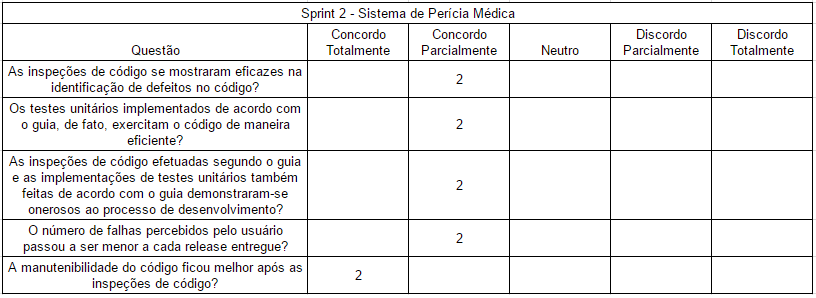
\includegraphics[width=\textwidth]{figuras/isd_pericia_2.png}
\caption{Índice de Satisfação dos Desenvolvedores - \textit{Sprint} 2 do Sistema de Perícia Médica}
\label{fig:satisfacaoPericia2}
\end{figure}

\clearpage

\section{Comparativo dos Ciclos}

A partir da execução de dois ciclos de pesquisa-ação foi possível perceber a mudança de opinião que as equipes de desenvolvimento apresentaram quanto à utilização do \textit{framework} de avaliação da qualidade de código.

No caso do projeto do Portal, após execução do segundo ciclo de pesquisa, foi possível perceber que 100\% dos desenvolvedores passaram a concordar totalmente com o aspecto de que a manutenibilidade do código passou a melhorar após realização de inspeções (questão 5). Adicionalmente, 100\% dos desenvolvedores passaram a concordar totalmente quanto à diminuição do número de falhas percebidas pelos usuários (questão 4).

A figura \ref{fig:evolucaoPortal} exibe dois gráficos comparativos, \textit{sprint} 1 e \textit{sprint} 2, que evidenciam as percepções dos desenvolvedores do Portal quanto ao uso do \textit{framework}. Apenas para fins de esclarecimento, as figuras exibem gráficos das duas \textit{sprints}, sendo os dados da \textit{sprint} 1 à esquerda e os dados da \textit{sprint} 2 à direita. As barras exibem a quantidade de respostas percebidas para cada questão (Q1, Q2, Q3, Q4 e Q5), bem como a classificação da resposta quanto à escala \textit{Likert}, sendo as abreviações:

\begin{itemize}
	\item CT - Concordo Totalmente
	\item CP - Concordo Parcialmente
	\item N - Neutro
	\item DP - Discordo Parcialmente
	\item DT - Discordo Totalmente
\end{itemize}

\begin{figure}[h]
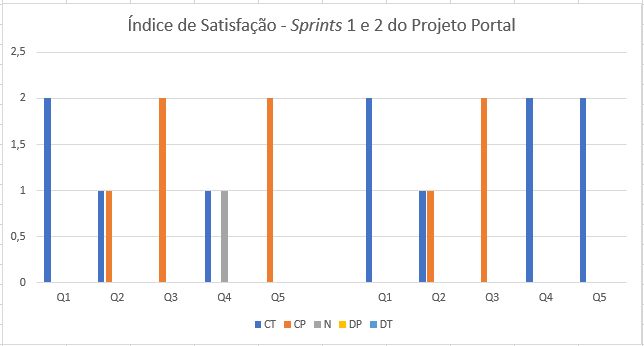
\includegraphics[width=\textwidth]{figuras/isd_portal.png}
\caption{Índice de Satisfação dos Desenvolvedores - Portal da Transparência - Evolução dos Ciclos}
\label{fig:evolucaoPortal}
\end{figure}

\hfill \break

\hfill \break

\hfill \break

\hfill \break

\hfill \break

\hfill \break

Com relação ao projeto SICOR, a equipe de desenvolvimento apresentou percepção similar à equipe do portal quanto ao aspecto de que as inspeções se mostraram eficientes na identificação de defeitos no código (questão 1), ou seja, 100\% dos desenvolvedores das duas equipes concordaram totalmente quanto a este aspecto em ambos os ciclos de pesquisa. Adicionalmente, ao final do ciclo 2, 100\% da equipe de desenvolvimento do SICOR passou a concordar totalmente quanto ao aspecto de que os testes unitários implementados de acordo com o guia proposto pelo \textit{framework} exercitam o código de maneira eficiente (questão 2).

A figura \ref{fig:evolucaoSicor} exibe dois gráficos comparativos, \textit{sprint} 1 e \textit{sprint} 2, que evidenciam as percepções dos desenvolvedores do SICOR quanto ao uso do \textit{framework}.

\begin{figure}[h]
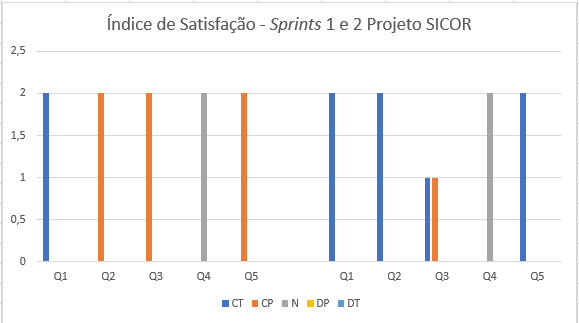
\includegraphics[width=\textwidth]{figuras/isd_sicor.png}
\caption{Índice de Satisfação dos Desenvolvedores - SICOR - Evolução dos Ciclos}
\label{fig:evolucaoSicor}
\end{figure}

\hfill \break

\hfill \break

\hfill \break

\hfill \break

\hfill \break

No caso do projeto Sistema de Perícia Médica, foi notória a evolução da percepção da equipe de desenvolvimento quanto à importância das práticas de verificação de \textit{software}. Para exemplificar essa afirmação, 100\% dos desenvolvedores eram neutros, no ciclo 1, quanto à eficácia das inspeções na identificação de defeitos e da utilidade dos testes unitários (questões 1 e 2). No ciclo 2, 100\% dos desenvolvedores passaram a concordar parcialmente quanto a estes aspecto. Contudo, desde o início, 100\% da equipe concordava totalmente quanto a melhoria da manutenibilidade após realização de inspeções (questão 5).

A figura \ref{fig:evolucaoPericia} exibe dois gráficos comparativos, \textit{sprint} 1 e \textit{sprint} 2, que evidenciam as percepções dos desenvolvedores do Sistema de Perícia Médica quanto ao uso do \textit{framework}.

\begin{figure}[h]
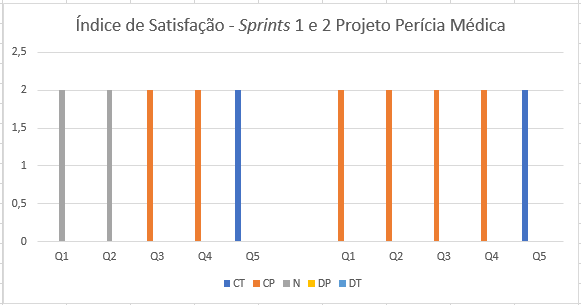
\includegraphics[width=\textwidth]{figuras/isd_pericia_medica.png}
\caption{Índice de Satisfação dos Desenvolvedores - Sistema de Perícia Médica - Evolução dos Ciclos}
\label{fig:evolucaoPericia}
\end{figure}

\hfill \break

\hfill \break

\hfill \break

\hfill \break

\hfill \break

Por fim, tem-se o gráfico geral para o projeto do Sistema de Ouvidoria. Neste caso, infelizmente não ocorreu a execução do segundo ciclo, mas é possível contemplar a receptividade dos desenvolvedores do mesmo quanto ao uso do \textit{framework} em uma iteração de desenvolvimento. A figura \ref{fig:evolucaoOuvdf} exibe o cenário geral.

\begin{figure}[h]
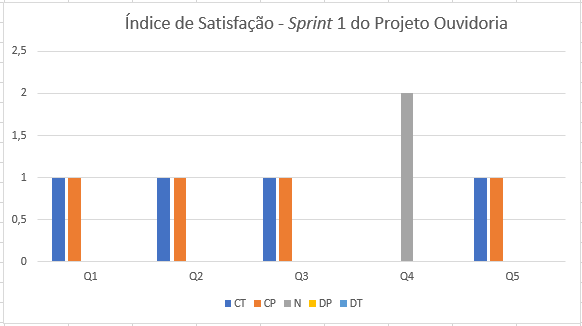
\includegraphics[width=\textwidth]{figuras/isd_ouvdf.png}
\caption{Índice de Satisfação dos Desenvolvedores - Sistema de Ouvidoria - Ciclo 1}
\label{fig:evolucaoOuvdf}
\end{figure}

Com base em todas as respostas coletadas, é possível perceber que não houve nenhuma resposta do tipo discordo totalmente ou discordo parcialmente. O \textit{framework}, de maneira geral, teve uma excelente aceitação e mostrou-se eficiente na verificação da qualidade.

\clearpage